\section{The CMS detector and Tau Reconstruction}
\begin{frame}{}
    \begin{center}
        \includegraphics[width=0.98\textwidth]{slides/figures/cmsDetector.png}
    \end{center}
\end{frame}

\begin{frame}{}
    \begin{center}
        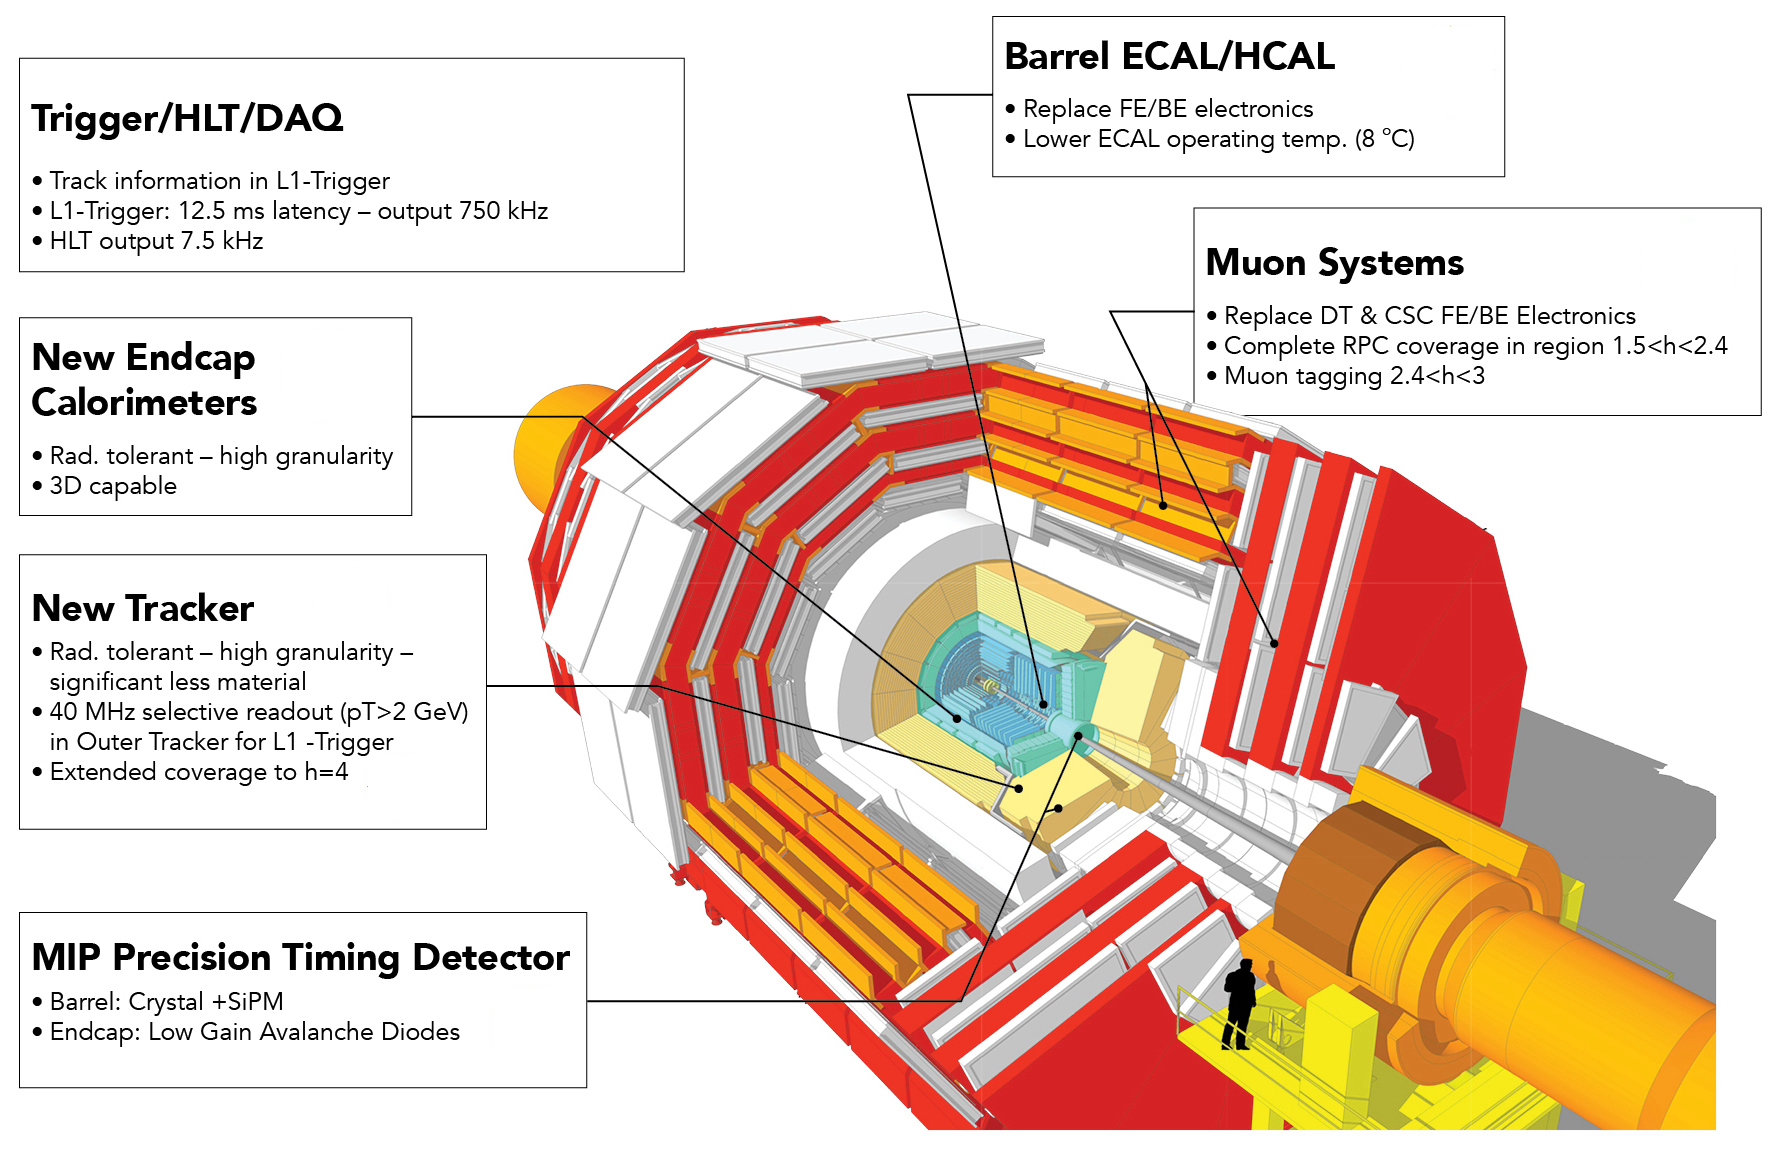
\includegraphics[width=0.98\textwidth]{slides/figures/CMS_NSF_DOE.jpeg}
    \end{center}
    The Phase-2 upgrade for the HL-LHC (2026-2035). \tiny{ https://www.classe.cornell.edu/NewsAndEvents/CLASSENewsCMS180129Ryan.html}
\end{frame}





% \begin{frame}{}
% \smaller
%     \begin{columns}
%     \column{0.6\textwidth}

%     \begin{itemize} 
%         \item Brain of the detector: Two-level trigger system.
%         \item level-1 trigger (L1T)
%         \begin{itemize} 
%             \item customized ASICs and onsite FPGAs
%             \item consider muon chamber and calorimeter
%             \item 40MHz to 100kHz
%             \item comprised of local, regional and global 
%             \item latency budget 4\mus 
%         \end{itemize}
        
%         \item high-level trigger (HLT)
%         \begin{itemize} 
%             \item CPU. commodity computers of builder-filter.
%             \item run a streamlined version of offline reconstruction software, filter with a HLT menu
%             \item 100\;kHz to 1\;kHz
%             \item in 2012, 13000 CPU cores 200 ms/event \cite{Trocino:2014jya}
%         \end{itemize}
%     \end{itemize}
    
    
%     \column{0.4\textwidth}
%     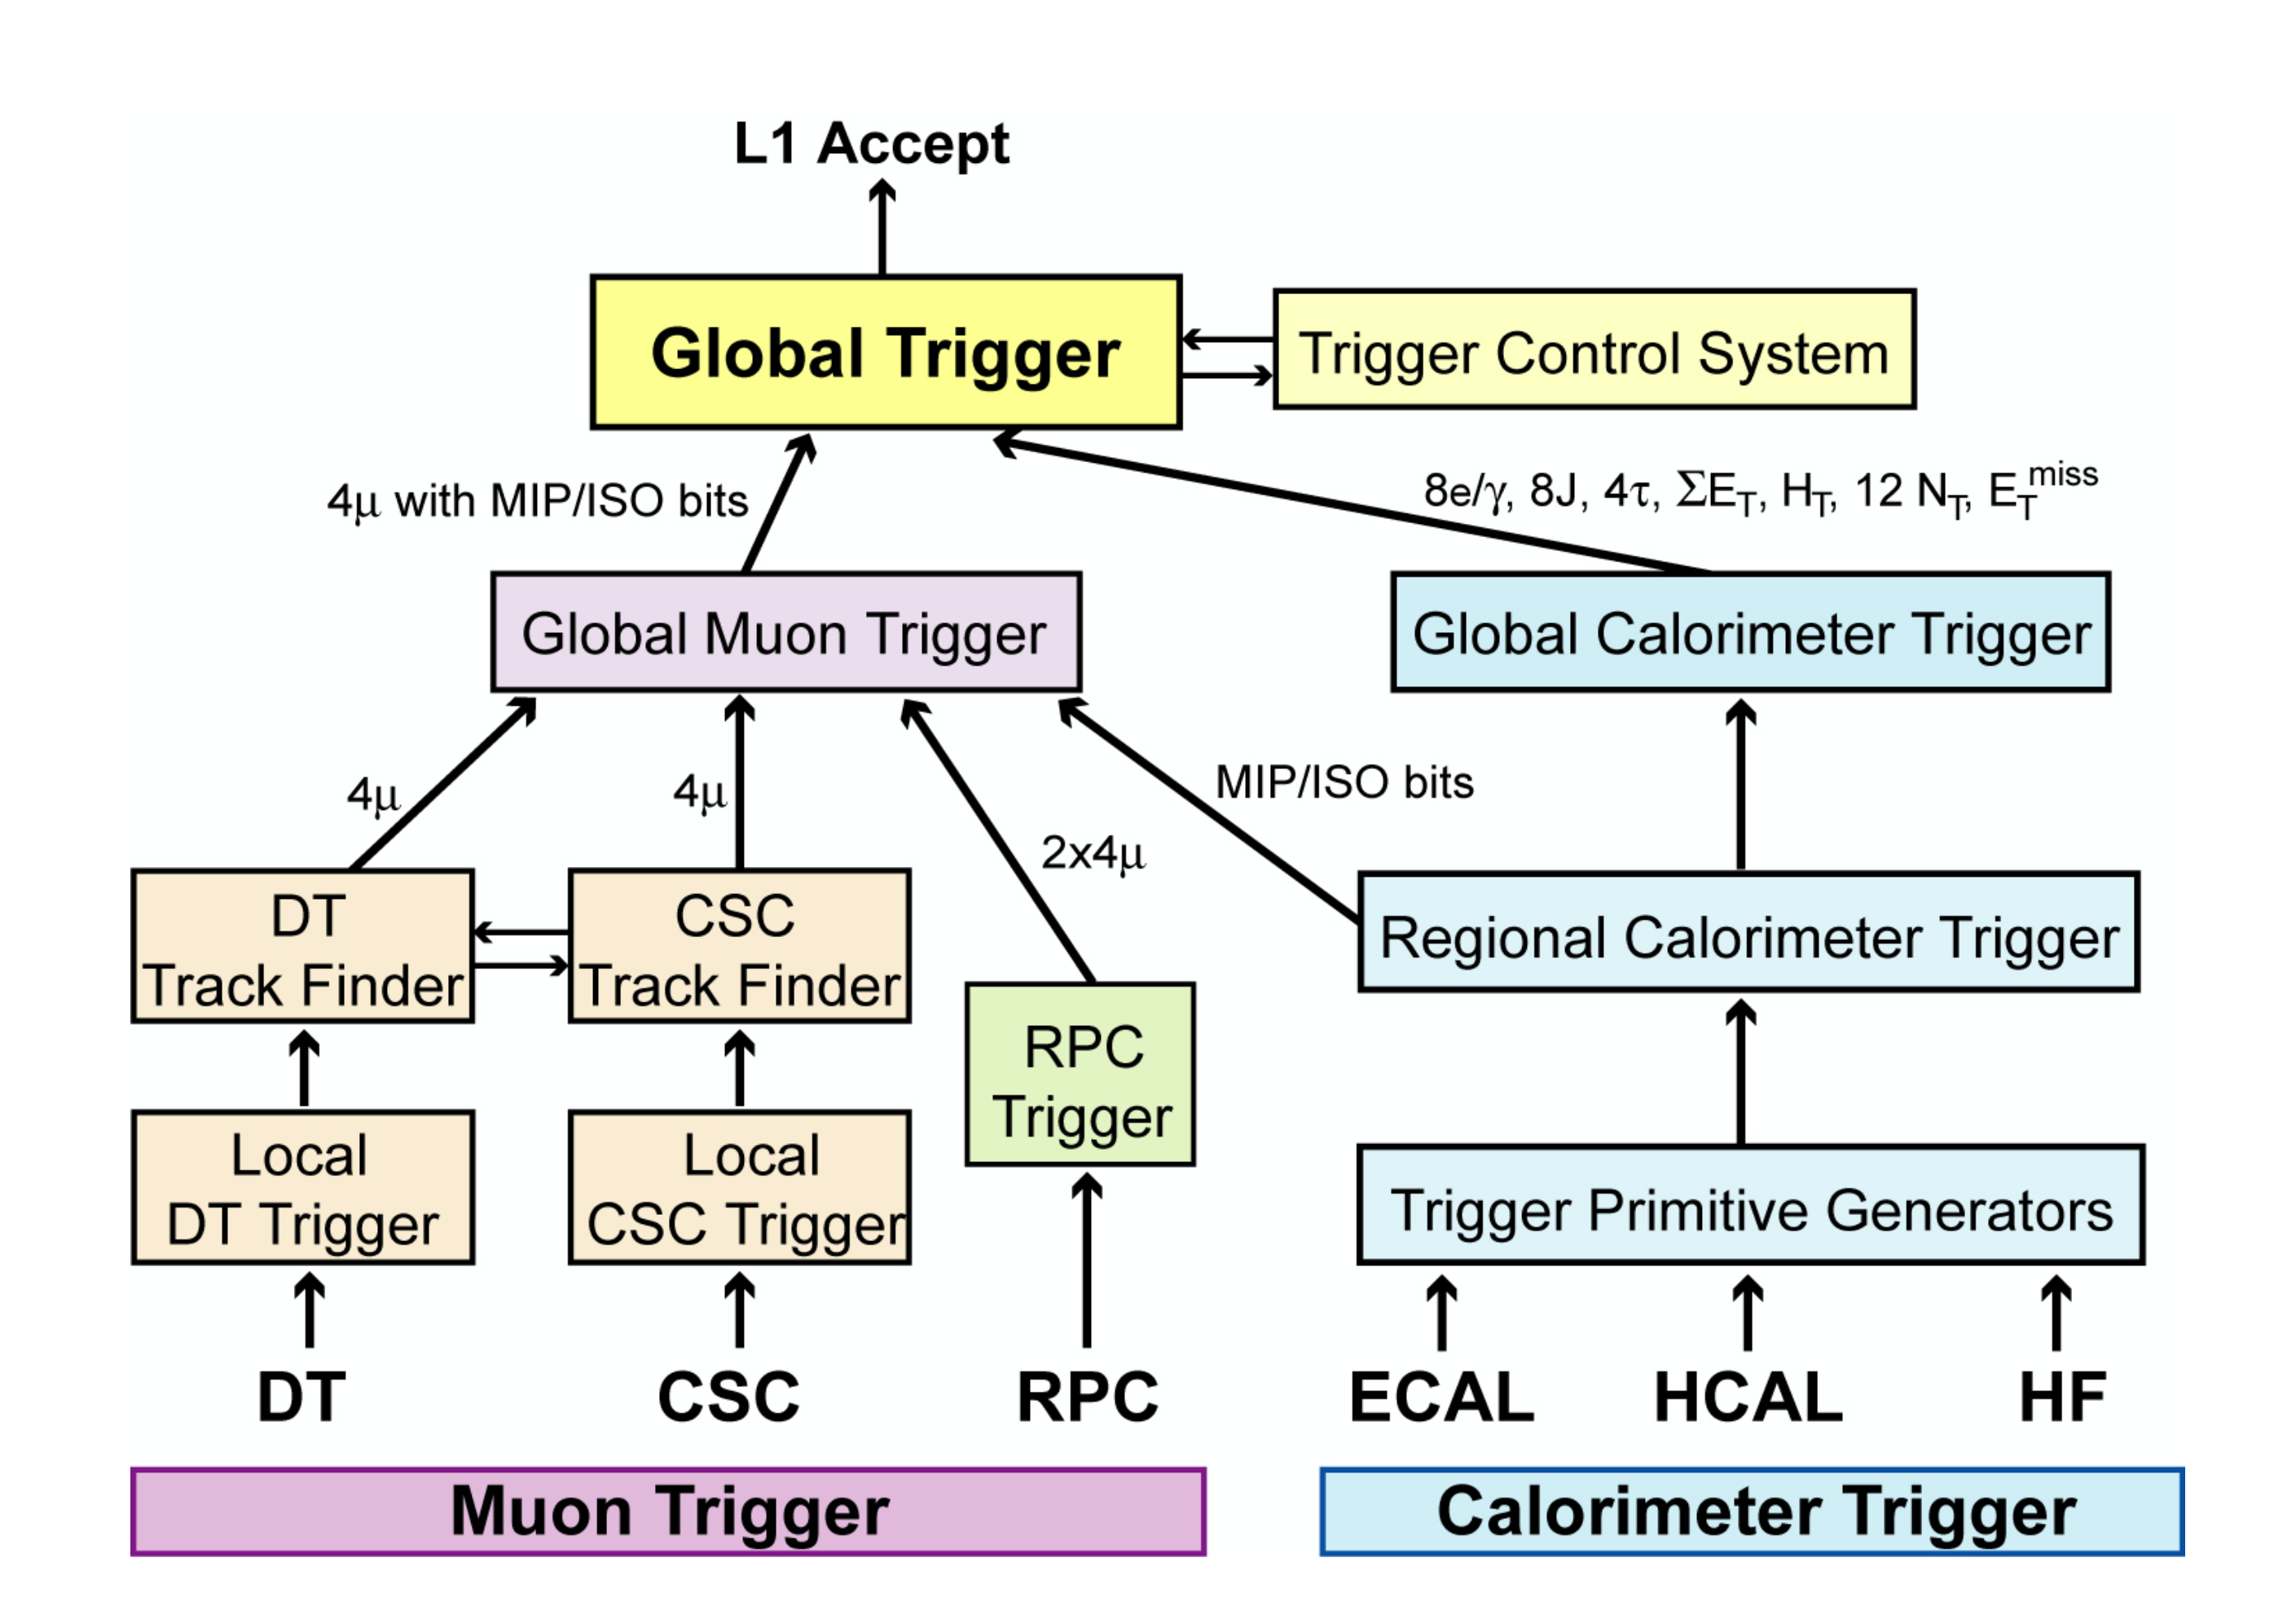
\includegraphics[width=\textwidth]{chapters/CMSExperiment/sectionTrigger/figures/trigger.png}
%     \end{columns}
% \end{frame}




\begin{frame}{High Granularity Calorimeter}
\smaller
    \begin{center}
        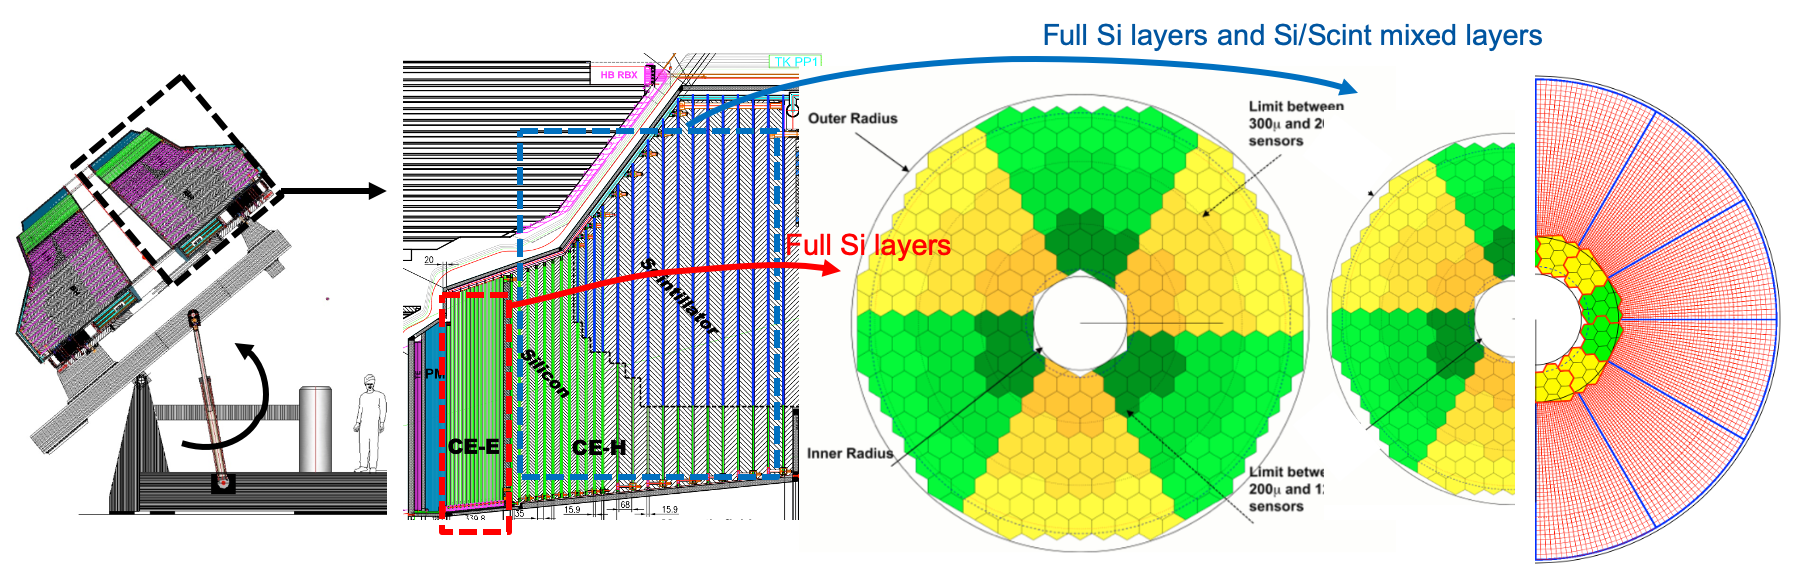
\includegraphics[height=0.32\textheight]{chapters/HGCal/figures/chep/hgcal2.png}
        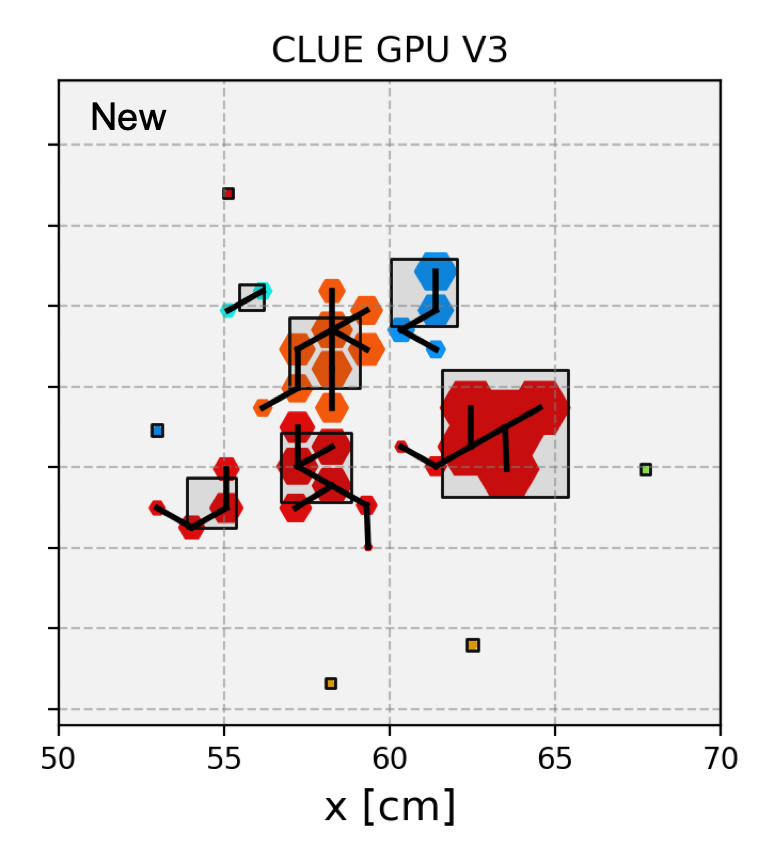
\includegraphics[height=0.3\textheight]{slides/figures/clue.png}
    \end{center}
    
    \begin{itemize} 
    \smaller
        \item A computing crisis: need 40x computing power (L1T 7.5x, high PU 3x, detector complexity 1.3x) 
        \item GPUs to be added to the CMS HLT computers.
        \item Work on HLT/Offline HGCAL reconstruction and its high performance computing with GPUs.
        \item Comparing with previous HGCAL clustering, CLUE gives exactly the same clustering results but is 200x faster (1000x if excluding data traffic/reformation time) 
    \end{itemize}
    
    \begin{center}
        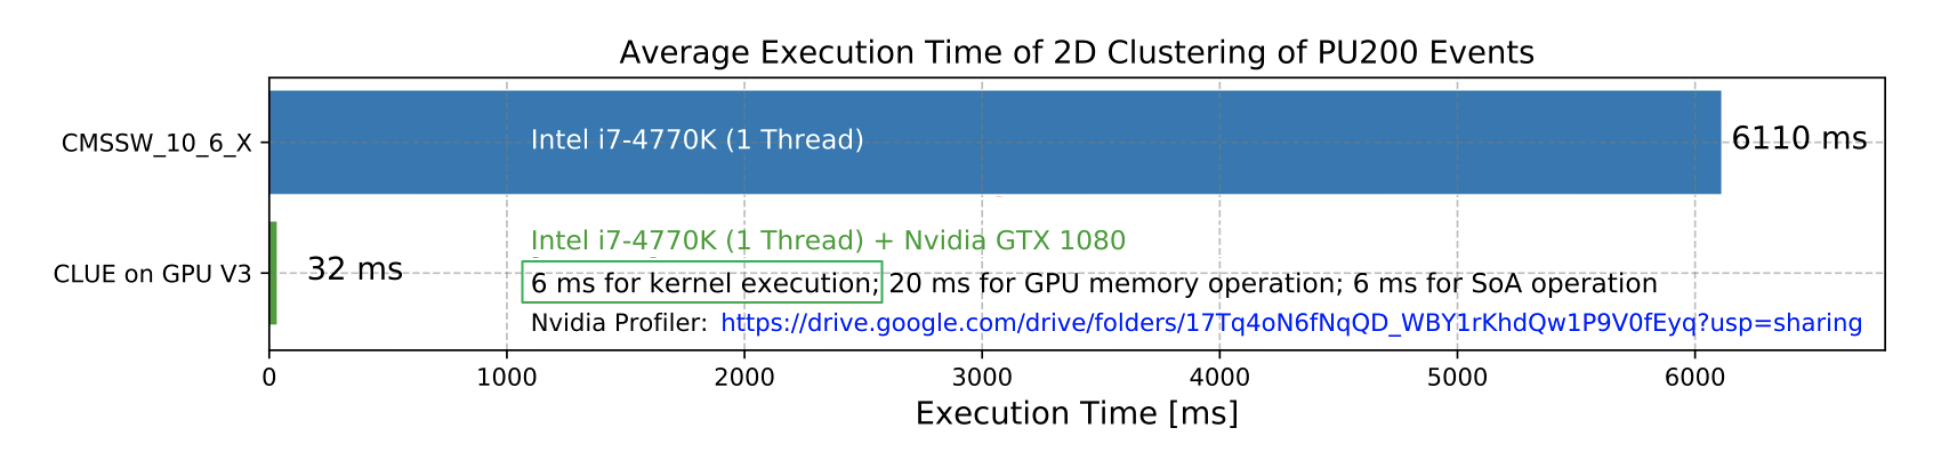
\includegraphics[width=0.99\textwidth]{slides/figures/clueTime.png}
    \end{center}
\end{frame}



\begin{frame}{Reconstruction with particle-flow}
\smaller
    \begin{center}
        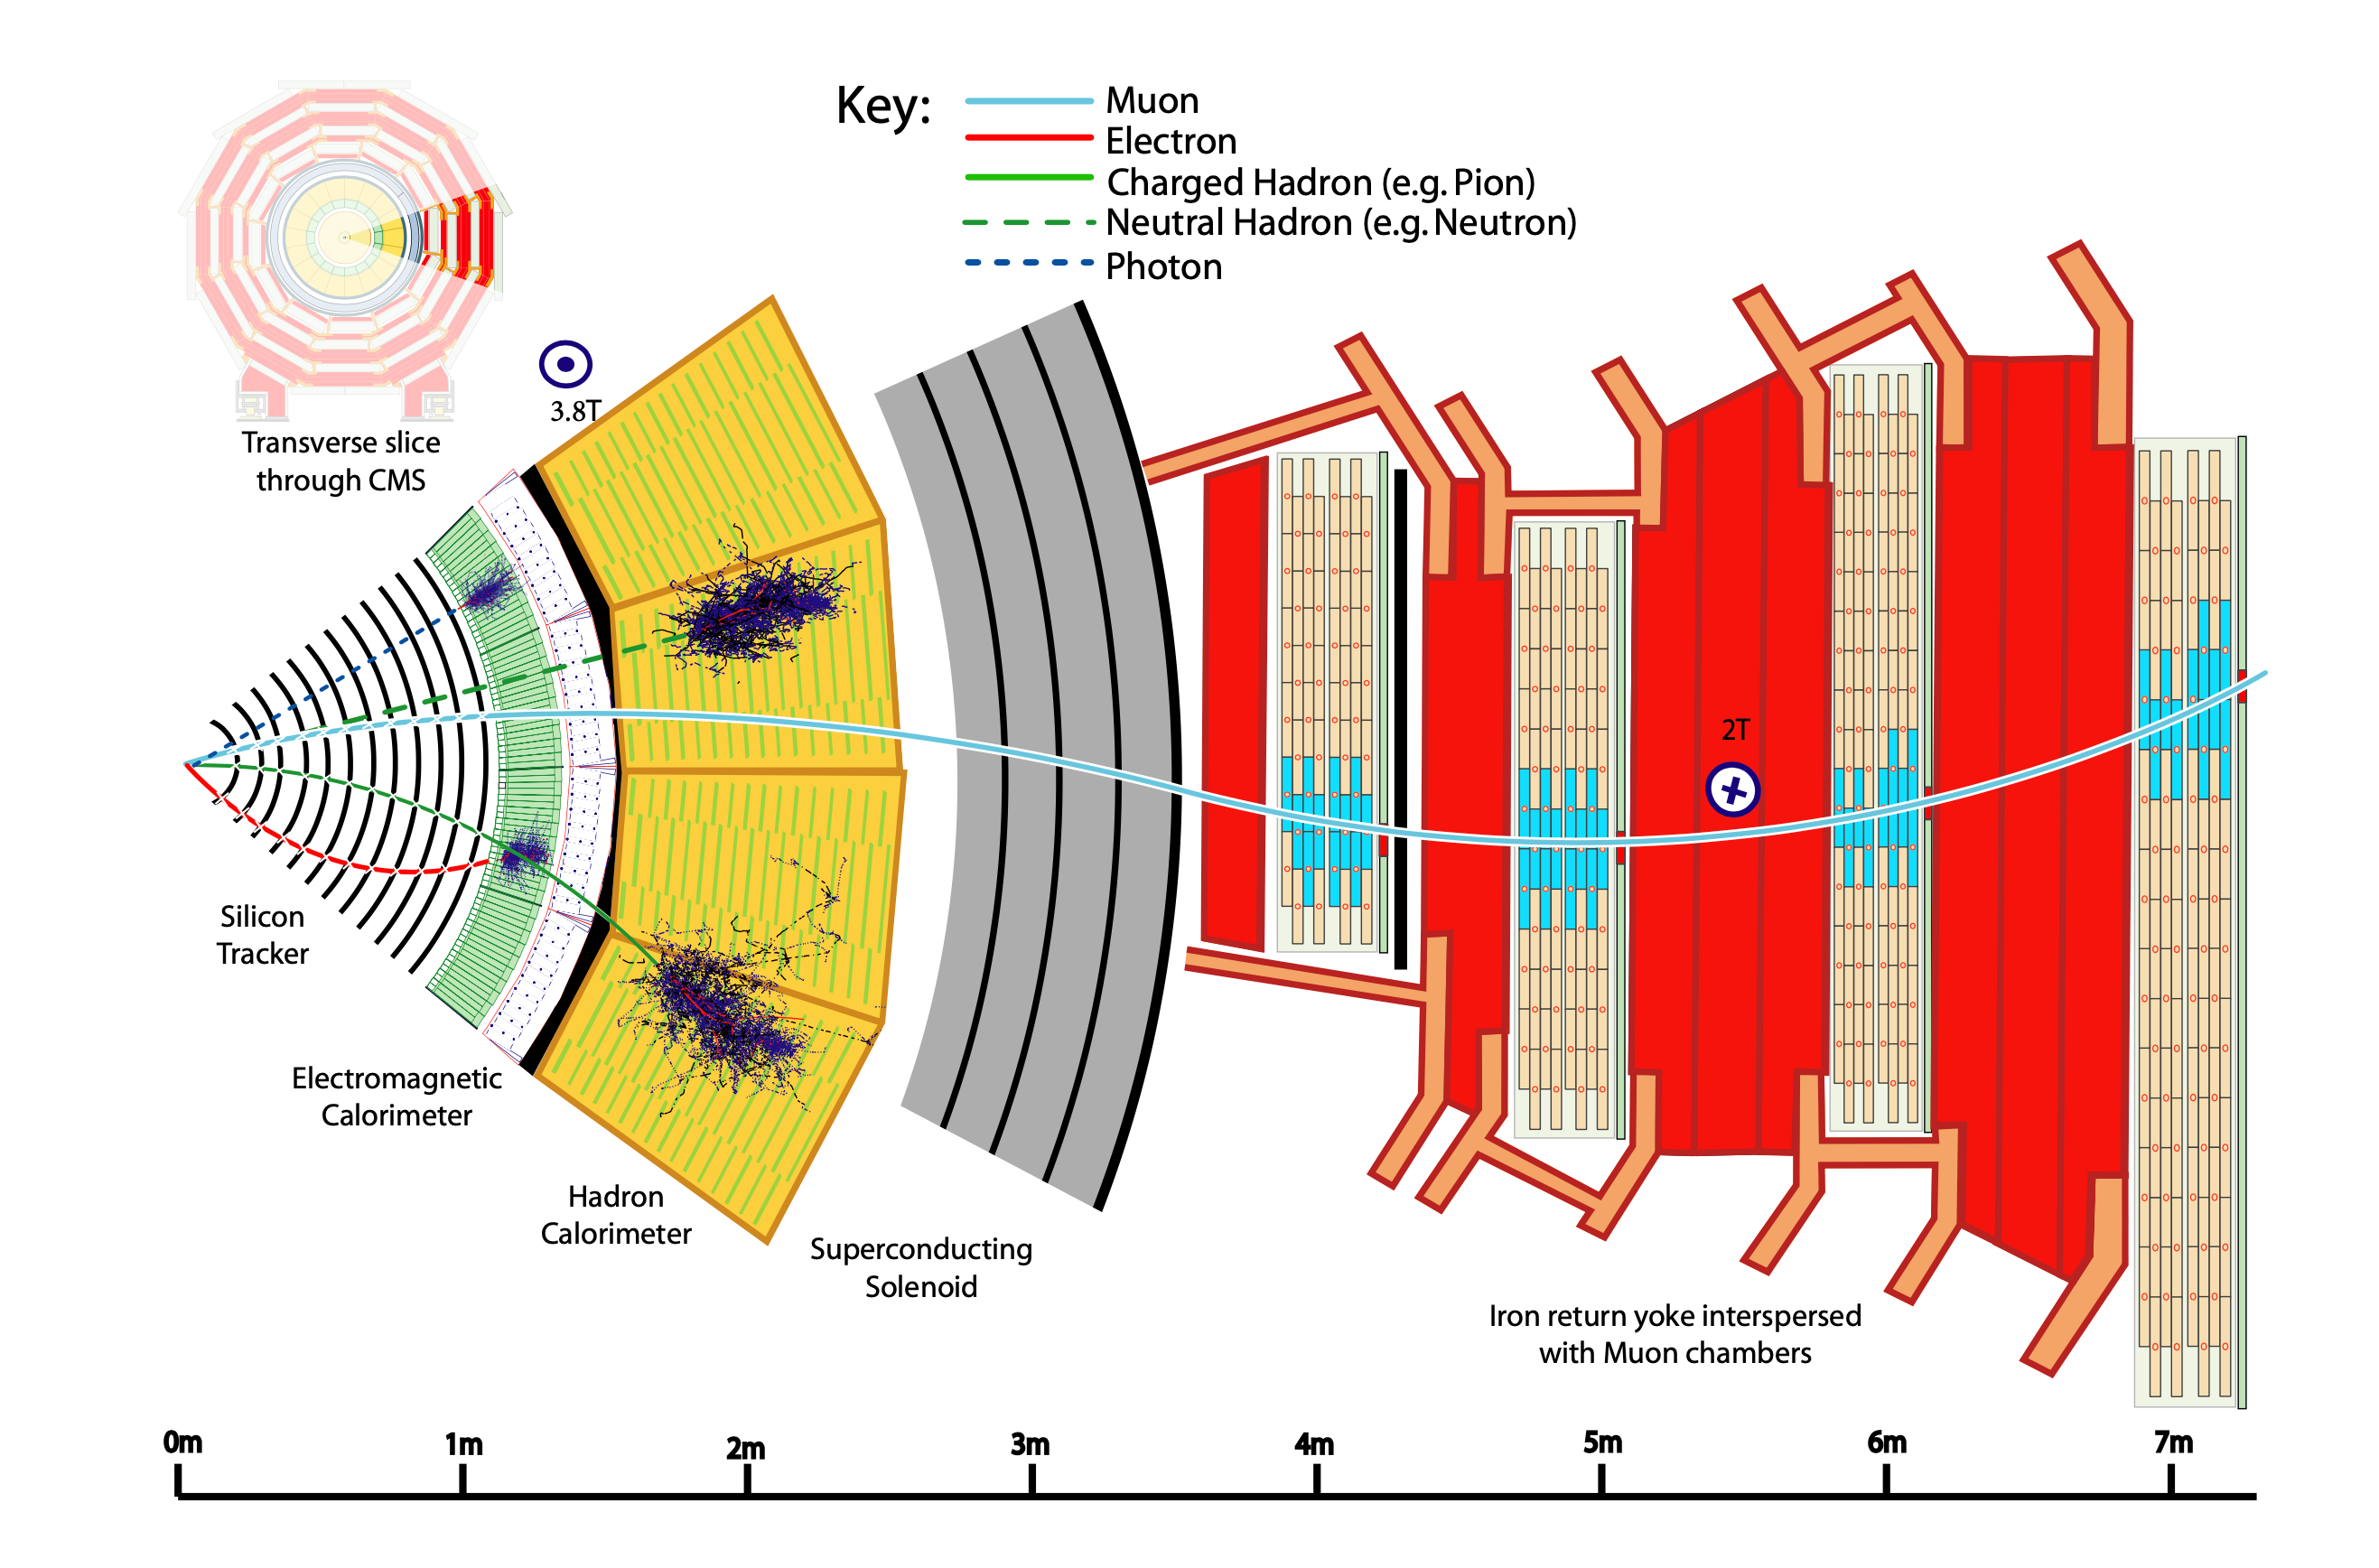
\includegraphics[width=0.7\textwidth]{chapters/CMSExperiment/sectionReconstruction/figures/pfa.png}
    \end{center}
    \begin{itemize} 
        \item Combines information from all sub-detectors to reconstruct final state particles (PF candidates). 
        \vspace{-0.05\textheight}
        \begin{itemize}
        \smaller
            \item \PGm, \Pe, $\mathrm{h}^{\pm}$, $\mathrm{h}^{0}$, \PGg
        \end{itemize}
        \item Main steps include building PF blocks, linking, identification/energy regression.
        \item Jets are made by clustering PF candidates with anti-\kt algorithm. 
        \item Jets originating from b quark and \textcolor{red}{\PGth} are tagged.
    \end{itemize}
\end{frame}

\begin{frame}{Hadronic tau reconstruction}
\smaller
    \begin{center}
        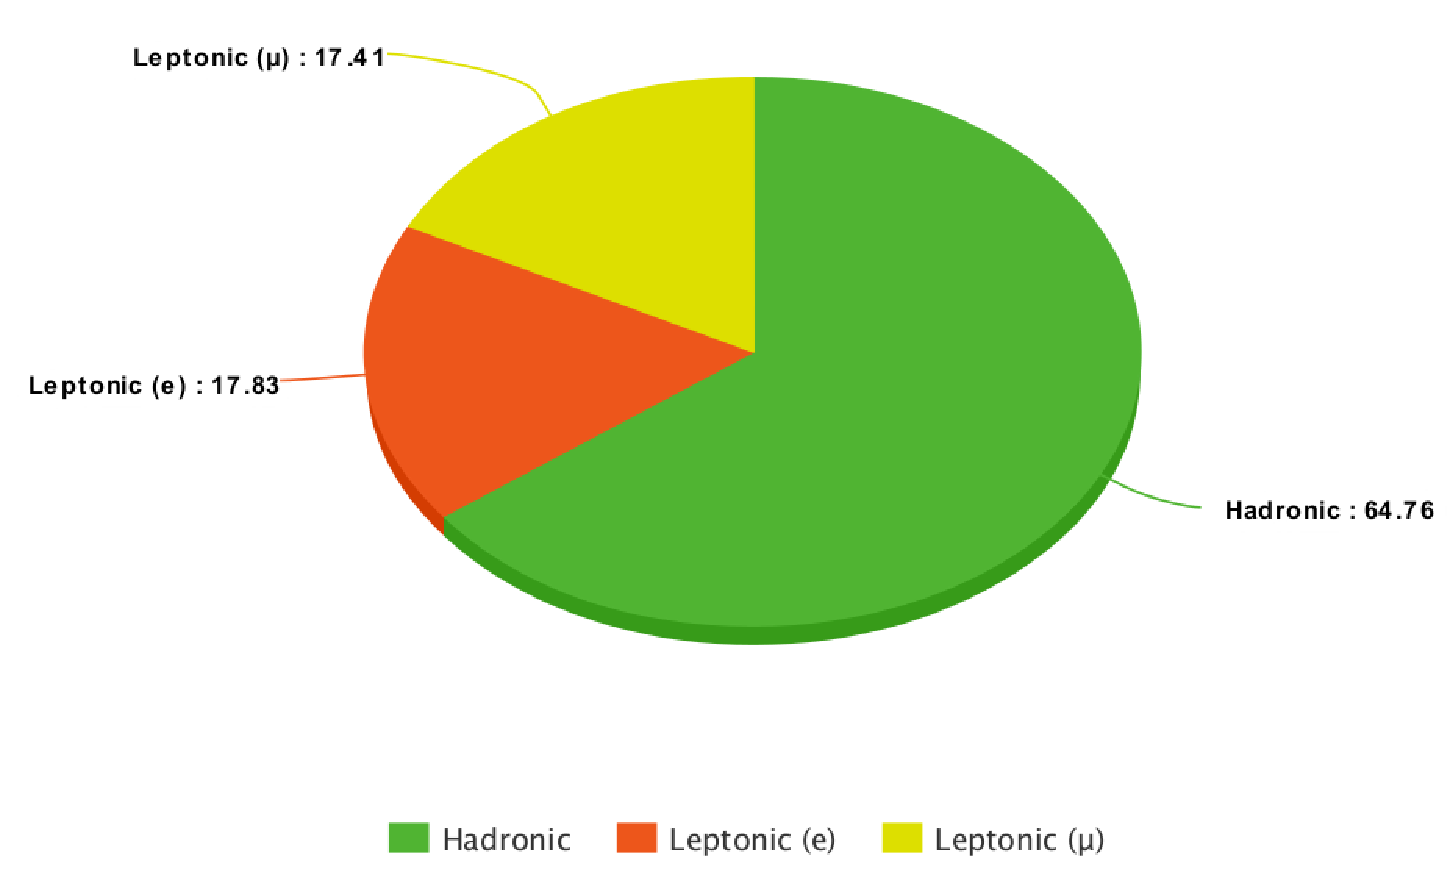
\includegraphics[height=0.4\textheight]{slides/figures/TauDecayPiChart.pdf}
        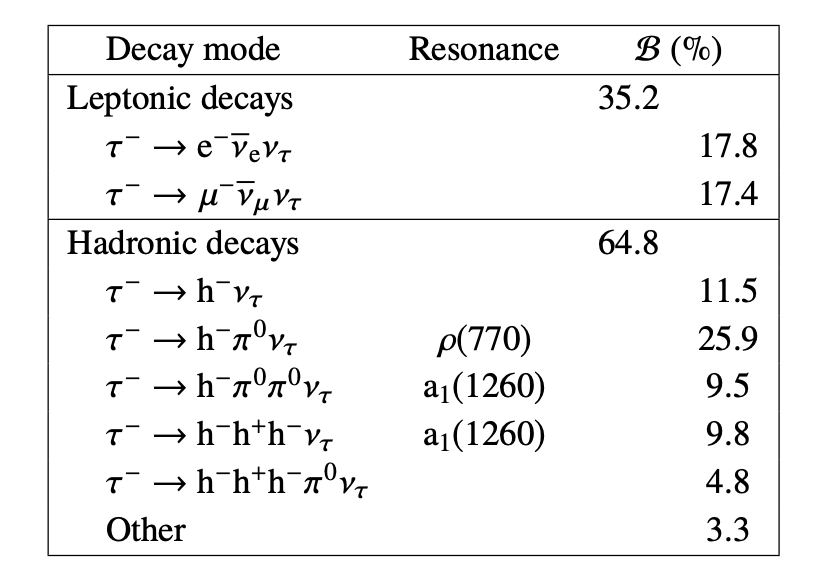
\includegraphics[height=0.4\textheight]{slides/figures/tauDecay.png}
    \end{center}
    \begin{block}{tau properties}
    \begin{itemize} 
        \item Mass $m_\PGt = 1.776\GeV$. Lifetime mean distance $c \cdot \Gamma = 87\mum$
        \item 65\% decay hadronically
        \item Hadronic decays have fixed patterns of final-state particles. 
        \item Exist well defined visible mass at $\rho (770)$ and $a_1(1260)$
    \end{itemize}  
    \end{block}
    In CMS, taus are reconstructed in their hadronic modes based on PF jets. 
\end{frame}

\begin{frame}{}
\smaller
    \begin{center}
        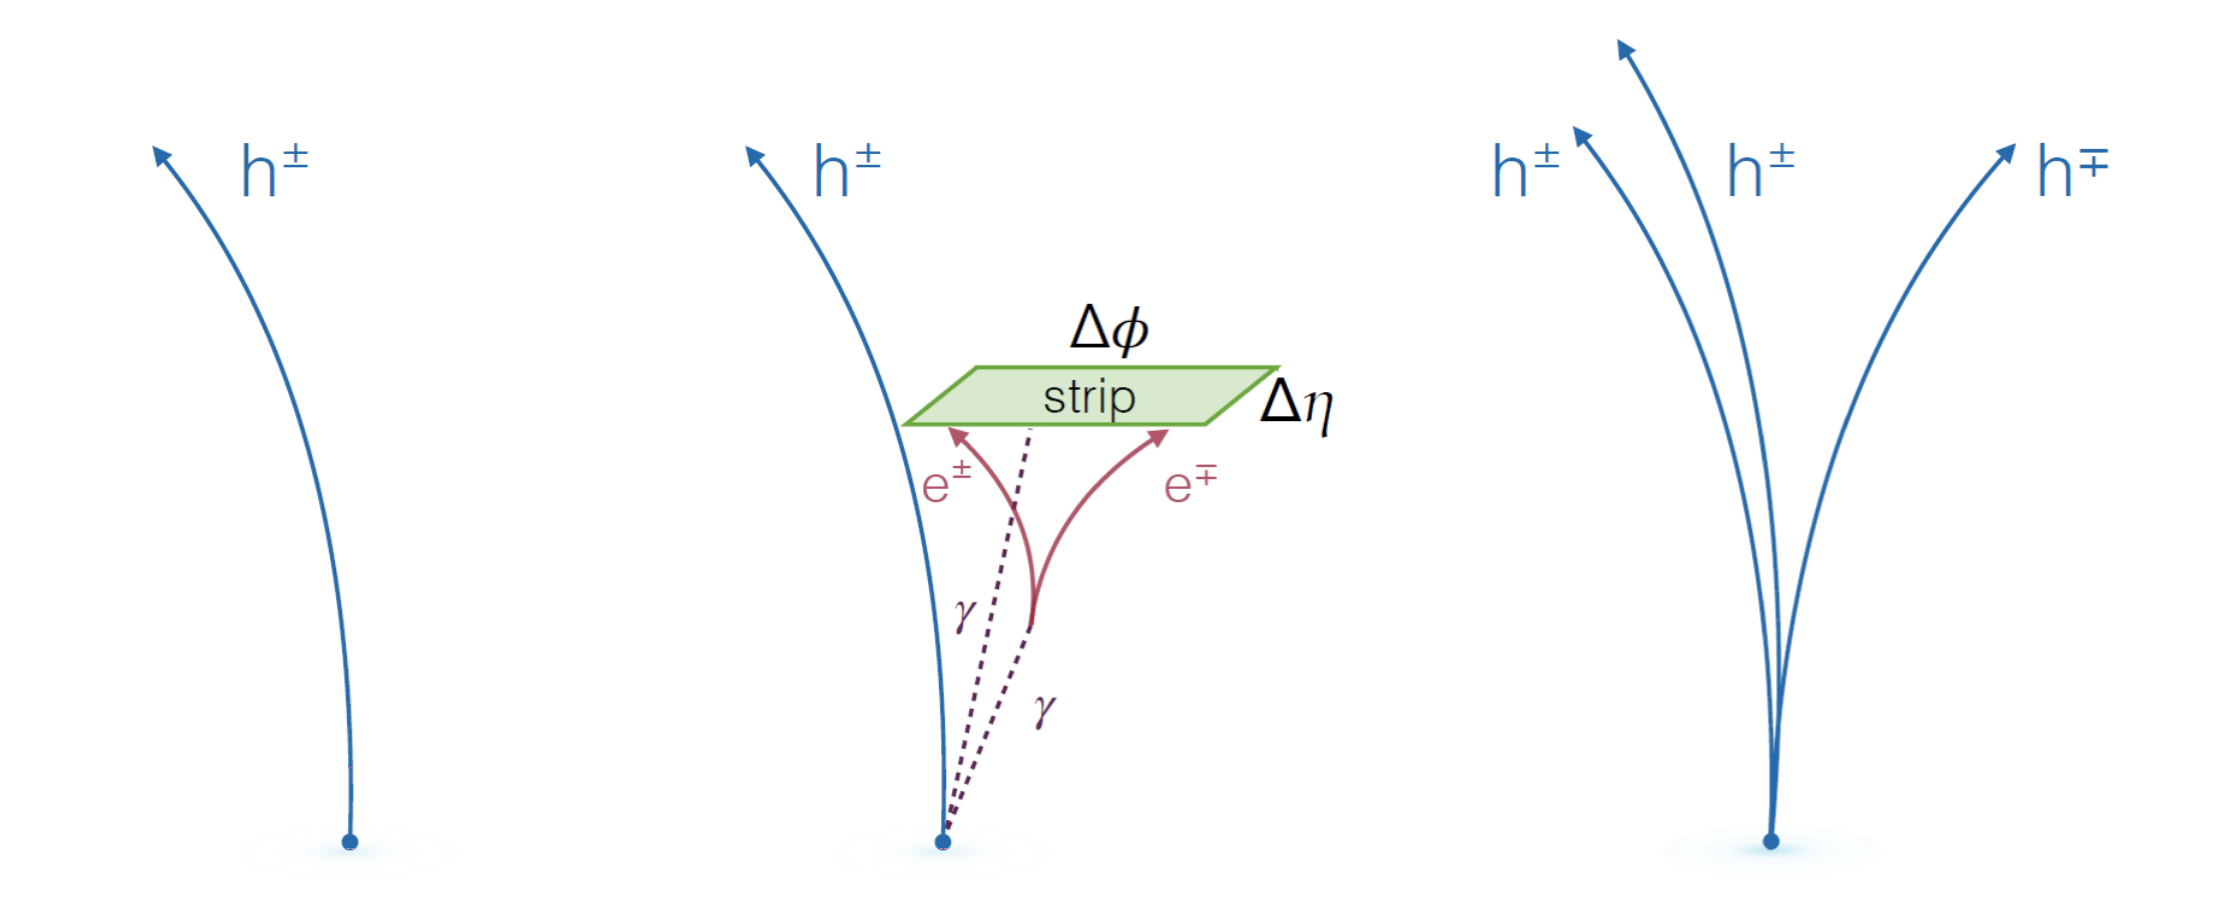
\includegraphics[width=0.6\textwidth]{slides/figures/tauReco.png}
    \end{center}
    \begin{block}{step-1 decay mode finding}
    Hadrons-plus-strips (HPS) algorithm is used to check the competence of jet structure to specific \PGth decay pattern.
    \begin{enumerate}
        \item cluster \Pe/\PGg into strips. merging \Pe/\PGg in \pt decreasing order with a dynamic window size $\Delta\eta \times \Delta \phi = 0.20\pt^{-0.66} \times 0.35 \pt^{-0.71}$ 
        \item select charged hadrons (prong) $\pt>0.5\GeV$ and $d_{xy}<0.1$~cm.
        \item match the hadrons-plus-strips to possible \PGth decay modes. ($h^-$, $h^- h^0$, $h^- h^+ h^-$ in 2016)
        \item veto when
        \begin{itemize} 
        \smaller
            \item not single charged
            \item visible mass not competent with expected $\rho (770)$ and $a_1(1260)$ resonance
            \item any hadrons or strips falls outside signal cone $\Delta R_{sig} = \frac{3.0 \text{ GeV } } { \pt (\text{ hadronic system})  }$, with $0.05 \leq \Delta R_{sig} \leq 0.1.$
        \end{itemize}
    \end{enumerate}  
    \end{block}
\end{frame}


\begin{frame}{}
\smaller
    
    \begin{columns}[c]
        \column{0.6\textwidth}
        \begin{block}{step-2 discriminate contaminations}
        \begin{itemize} 
            \item discriminate against quark and gluon jets.
            \item iso-based discriminator: 
            \begin{itemize} 
            \smaller
                \item isolation is calculated energy sum in the ring between signal cone and $\Delta R = 0.3$ cone.
                \item quark and gluon jets tend to have larger isolation, while tau jets tend to have smaller.
            \end{itemize}
        
             
            % \begin{equation}
            % \tiny
            %     I_{\PGth} = \sum \pt^{\text{charged}} (d_z<0.2 \text{cm}) + \max \bigg( 0, \sum \pt^ \PGg - \Delta \beta \sum \pt^{\text{charged}} (d_z>0.2 \text{cm})  \bigg )
            % \end{equation}
            
            \item MVA-based discriminator: 
            \begin{itemize} 
            \smaller
                \item combine isolation and other variables sensitives to tau lifetime (e.g. SIP3D, d0).
                \item use boosted decision tree (BDT)
            \end{itemize}
            
            
        \end{itemize}
        \end{block}

        \column{0.4\textwidth}
        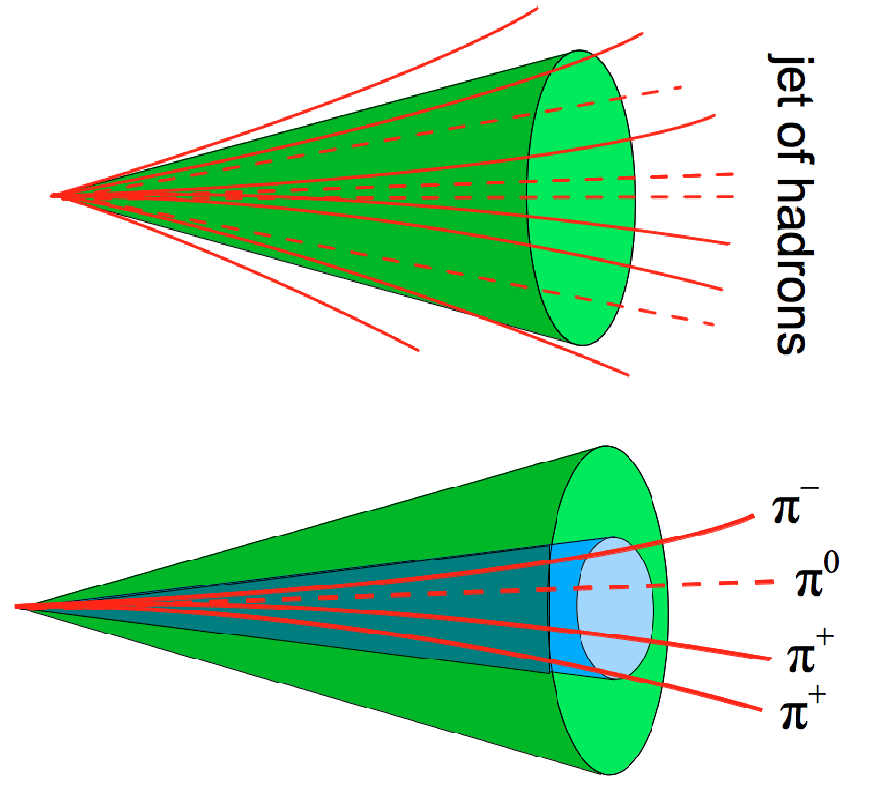
\includegraphics[width=\textwidth]{slides/figures/tausignature_trans.png}
    \end{columns}
    
\end{frame}